\documentclass{article}
\usepackage{tikz}

\begin{document}

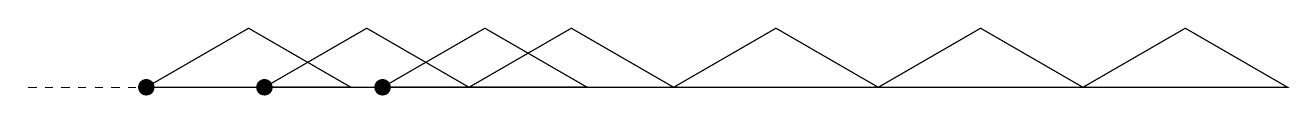
\begin{tikzpicture}[scale=1.5]
    % Draw the horizontal line
    \draw[dashed] (-2,0) -- (2,0);
    
    % Define coordinates for the points
    \coordinate (A) at (-1,0);
    \coordinate (B) at (0,0);
    \coordinate (C) at (1,0);
    
    % Draw the first triangle
    \draw (A) -- ++(30:1) coordinate (A1) -- ++(-30:1) coordinate (A2) -- cycle;
    
    % Draw the second triangle
    \draw (B) -- ++(30:1) coordinate (B1) -- ++(-30:1) coordinate (B2) -- cycle;
    
    % Draw the third triangle
    \draw (C) -- ++(30:1) coordinate (C1) -- ++(-30:1) coordinate (C2) -- cycle;
    
    % Draw the zigzag pattern
    \draw (B2) -- ++(30:1) coordinate (B3) -- ++(-30:1) coordinate (B4) -- cycle;
    \draw (B4) -- ++(30:1) coordinate (B5) -- ++(-30:1) coordinate (B6) -- cycle;
    \draw (B6) -- ++(30:1) coordinate (B7) -- ++(-30:1) coordinate (B8) -- cycle;
    \draw (B8) -- ++(30:1) coordinate (B9) -- ++(-30:1) coordinate (B10) -- cycle;
    
    % Draw the dots at the vertices
    \fill (A) circle (2pt);
    \fill (B) circle (2pt);
    \fill (C) circle (2pt);
\end{tikzpicture}

\end{document}